%!TEX root = ./main.tex
\section{Results}
This section describes the results to our research questions aimed at understanding the types of refactoring developers apply the most on test code as well as their impact on production code maintainability. 

\noindent
\subsection*{RQ1: What type of refactorings do developers apply on test code?}
To find what types of refactorings developers apply the most on test code, we used Refactor-miner on our subject systems. The results can be found in Table~\ref{table:9}.
% \ifx true false

% \begin{table}[!ht]
% \centering
% \begin{tabular}{|l|l|l|l|}
% \hline
% \multicolumn{4}{|c|}{Sonarqube} \\ \hline
% Extract Method & 315 & Pull Up Attribute & 33 \\ \hline
% Move Class & 1118 & Extract Superclass & 12 \\ \hline
% Move Attribute & 341 & Push Down Method & 37 \\ \hline
% Rename Package & 6 &  Push Down Attribute & 3 \\ \hline
% Move Method & 553 & Extract Interface & 1 \\ \hline
% Inline Method & 53 & Rename Class & 820 \\ \hline
% Pull Up Method & 59 & Rename Method & 3481 \\ \hline
% \end{tabular}
% \caption{Amount of refactorings by type in sonarqube}
% \label{table:9}
% \end{table}

% \begin{table}[!ht]
% \centering
% \begin{tabular}{|l|l|l|l|}
% \hline
% \multicolumn{4}{|c|}{Hadoop} \\ \hline
% Extract Method & 1690 & Pull Up Attribute & 152 \\ \hline
% Move Class & 261 & Extract Superclass & 46 \\ \hline
% Move Attribute & 395 & Push Down Method & 2 \\ \hline
% Rename Package & 0 &  Push Down Attribute & 0 \\ \hline
% Move Method & 721 & Extract Interface & 3 \\ \hline
% Inline Method & 89 & Rename Class & 555 \\ \hline
% Pull Up Method & 175 & Rename Method & 1363 \\ \hline
% \end{tabular}
% \caption{Amount of refactorings by type in hadoop}
% \label{table:10}
% \end{table}

% \begin{table}[!ht]
% \centering
% \begin{tabular}{|l|l|l|l|}
% \hline
% \multicolumn{4}{|c|}{Elasticsearch} \\ \hline
% Extract Method & 565 & Pull Up Attribute & 23 \\ \hline
% Move Class & 1363 & Extract Superclass & 73 \\ \hline
% Move Attribute & 282 & Push Down Method & 298 \\ \hline
% Rename Package & 6 &  Push Down Attribute & 100 \\ \hline
% Move Method & 1071 & Extract Interface & 0 \\ \hline
% Inline Method & 57 & Rename Class & 2401 \\ \hline
% Pull Up Method & 311 & Rename Method & 4370 \\ \hline
% \end{tabular}
% \caption{Amount of refactorings by type in elasticsearch}
% \label{table:11}
% \end{table}

% \fi

\begin{table}[!ht]
\caption{Refactorings by type in the subject systems.}
\label{table:9}
\resizebox{\columnwidth}{!}{%
\begin{tabular}{lrrrrrr}
\hline
 & Sonarqube & Hadoop & Elasticsearch & Total \\ \hline
Rename Method & 3481 & 1363 & 4370 & 9214 \\
Move Class & 1118 & 261 & 1363 & 2742 \\
Rename Class & 820 & 555 & 2401 & 3776 \\
Move Method & 553 & 721 & 1071 & 2345 \\
Move Attribute & 341 & 395 & 282 & 1018 \\
Extract Method & 315 & 1690 & 565 & 2570 \\
Pull Up Attribute & 33 & 152 & 23 & 208 \\
Extract Superclass & 12 & 46 & 73 & 131 \\
Push Down Method & 37 & 2 & 298 & 337 \\
Rename Package & 6 & 0 & 6 & 12 \\
Push Down Attribute & 3 & 0 & 100 & 103 \\
Extract Interface & 1 & 3 & 0 & 4 \\
Inline Method & 53 & 89 & 57 & 199 \\
Pull Up Method & 59 & 175 & 311 & 545 \\
\end{tabular}
}
\end{table}

\begin{figure}[!ht]
 \centering
 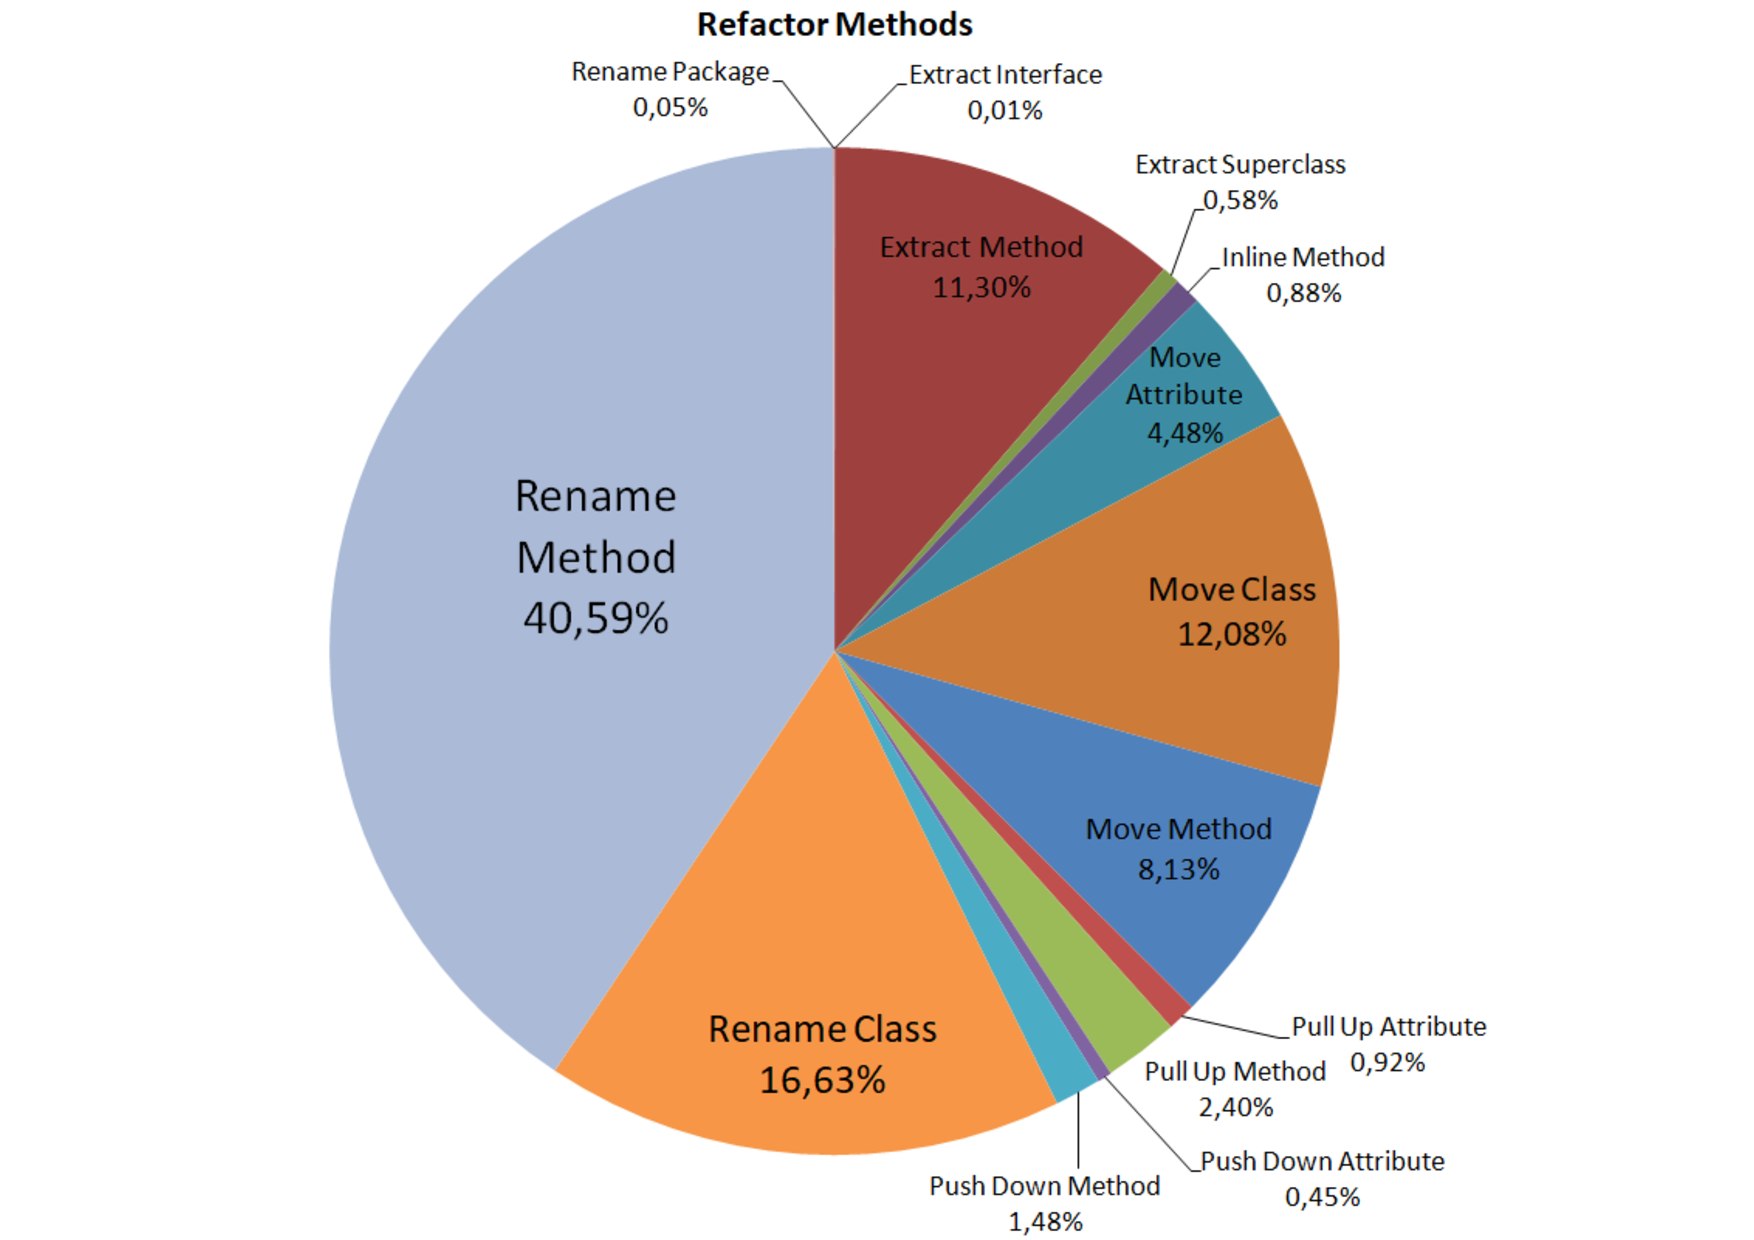
\includegraphics[width=\columnwidth]{resources/refactorMethods.pdf}
 \caption{Percentages of the refactor methods of all the repositories}
 \label{figure:piechart}
\end{figure}

As we can notice, some refactor methods were used more often than others. The most popular refactor method for test code would be \textit{Rename Method}. The refactor methods \textit{Rename Class}, \textit{Move Class} and \textit{Extract Method} were also used often. These methods are used for improving the names and location of codes, but also for giving the code a more logical structure. Refactor methods like \textit{Rename Package}, \textit{Extract Interface}, \textit{Extract Superclass}, \textit{Push Down Method} and \textit{Push Down Attribute} were instead barely used. Another result we can notice is that some of the refactor methods were used much more in a project than in the others. For instance, \textit{Extract Method} was used much more in the Hadoop than in Sonarqube or Elasticsearch. We speculate that this might happen because each project has their own "rules of code quality" that developers have to apply, as well as their own ideas about refactoring code (for example, some projects can have more strict rules and force developers to refactor test code).

Given our experimental setting, we cannot speculate on the motivations behind the results achieved so far: indeed, our RQ$_1$ meant to be a coarse-grained investigation aimed at understanding what types of refactorings developers apply the most. Thus, in this research question we did not focus on the reasons behind these refactorings, \eg are the test refactored due to a change in the production code? or maybe because developers were close to a new release? Our RQ$_3$ makes a first step in providing additional insights on such a relationship, however further research should better investigate this relationship.

%In the \textit{Sonarqube} project, the refactor method \textit{Rename Method} seems to be used far more often than in the \textit{Hadoop} project. The same can be said about the refactor method \textit{Extract Method}, which is used far more often in the Hadoop project as in the Sonarqube project. Ofcourse, each project has its own difficulties and thereby their own refactorings. 

%-----------------------------------------------------------------------------------------------
% \subsection*{RQ2: Does the refactoring of test code affect the maintainability of production code?}\label{maintainability:improved}
% In this section we want to adres the results found that have been collected in an attempt to answer RQ2. Refactor data on test classes has been gathered and their matching production classes were checked every 10 commits after that for 5 versions in total, so up to 50 commits ahead. As mentioned in the explanation of RQ2 we will be looking at refactors on test code that significantly improved the maintainability of that test class. We define a significant improvement as a summed difference in the classes each metric among LOC, NOF, NOM and WMC. An example, a class that went from Medium to Low in terms of LOC, has a difference of 1 in terms of LOC. High to Very Low is a difference of 4, Low to High is a difference of -2. Adding the difference for each metric gives us the summed difference, if this value exceeds 4 we say the improvement is significant.  Among all projects we have found the follwing numbers:
% \begin{table}[!ht]
%     \centering
%     \begin{tabular}{|l|l|}
%         \hline
%         \multicolumn{2}{|c|}{Test refactorings} \\ \hline
%         Total & 1756 \\ \hline
%         Worsened & 236 \\ \hline
%         Unaffected & 824 \\ \hline
%         Improved & 696 \\ \hline
%         Significantly improved & 108 \\ \hline
%     \end{tabular}
%     \caption{Counts of test refactorings and how they affected maintainability}
%     \label{table:12}
% \end{table}
% We then check the first and last version of the matching production class that was tracked and calculate the difference here as well. Some production files could not be tracked, this can be accounted to rename or deletions of the file causing our code to be unable to find the file.
% \begin{table}[!ht]
%     \centering
%     \begin{tabular}{|l|l|}
%         \hline
%         \multicolumn{2}{|c|}{Tracked production files} \\ \hline
%         Total & 108 \\ \hline
%         Affected & 0 \\ \hline
%         Unaffected & 85 \\ \hline
%         Error in tracking & 23 \\ \hline
%     \end{tabular}
%     \caption{Tracked production files' maintainability after significant maintainability improving test refactor}
%     \label{table:13}
% \end{table}
% Surprising not a single production file was modified significantly (i.e. causing a shift in its classification among the metrics we look at). Suggesting that it is very unlikely that a refactoring in test code that significantly improves maintainability causes a similar improvement in the production class under test. Now this result is not what we were expecting, now this is also something that might be related to the projects under analysis, updating test code might not happen before updating the production class, perhaps it is the other way around, production code first, after which test code gets updated. Perhaps it happens more in a periods of pure testing and pure development, such period have also been identified by \cite{zaidman2008mining}. This way our method by looking up to 50 commits in the future after a test code refactoring, does not find the corresponding production file change, if present at all. On the other hand if testing and development are done in different periods then we cannot accredit a test code refactoring to cause a change in production code.

%-----------------------------------------------------------------------------------------------
\subsection*{RQ2: What is the correlation between test code maintainability and production code maintainability?}
\label{maintainability:correlation}
Using the categories defined in Section~\ref{sec:maint-metric}, we have categorized the risk for each pair Production-Test class for all the metrics. As shown in Table~\ref{table:6}, we mined a total of 177 snapshots: Since plotting all the snapshots would result in too much data, we have chosen to visualise only 5 snapshots (randomly selected) for each project, hence 15 in total. 

In Figure~\ref{fig:heat_map} we show the result. On the axis we can find the risk categories: The X-axis shows the category in which the test class is classified, while the Y-axis shows the category of the corresponding production class. 

\subsubsection{Analyzing the results}
Throughout all the metrics we have analyzed in every project we see a strong correlation in production and test classes both being classified in the Very Low risk category. This correlation is not that present in the other categories, and this holds for each metric. We do however notice a high density in the leftmost column in each plot: This indicates that where production classes are being classified in a variety of categories, the vast majority of test classes is classified in the Very Low risk category. This can be attributed to the general lower complexity of a test class compared to a production class. For example, a highly complex production class can still be tested with a relatively simple test class that verifies if the output of certain functions is as expected.

The high density in the Very Low category for both test and production classes is a surprising result: for each of these metrics it holds that where a production class is categorized as low risk, so is the corresponding test class, giving an indication that a relation is present. However we do not see this density in the "Low/Low", "Medium/Medium" and "High/High" categories: As previously discussed, this can be led back to the argument presented earlier, that even higher complexity classes can be tested using relatively simple test classes.

\begin{figure*}
    \centering
    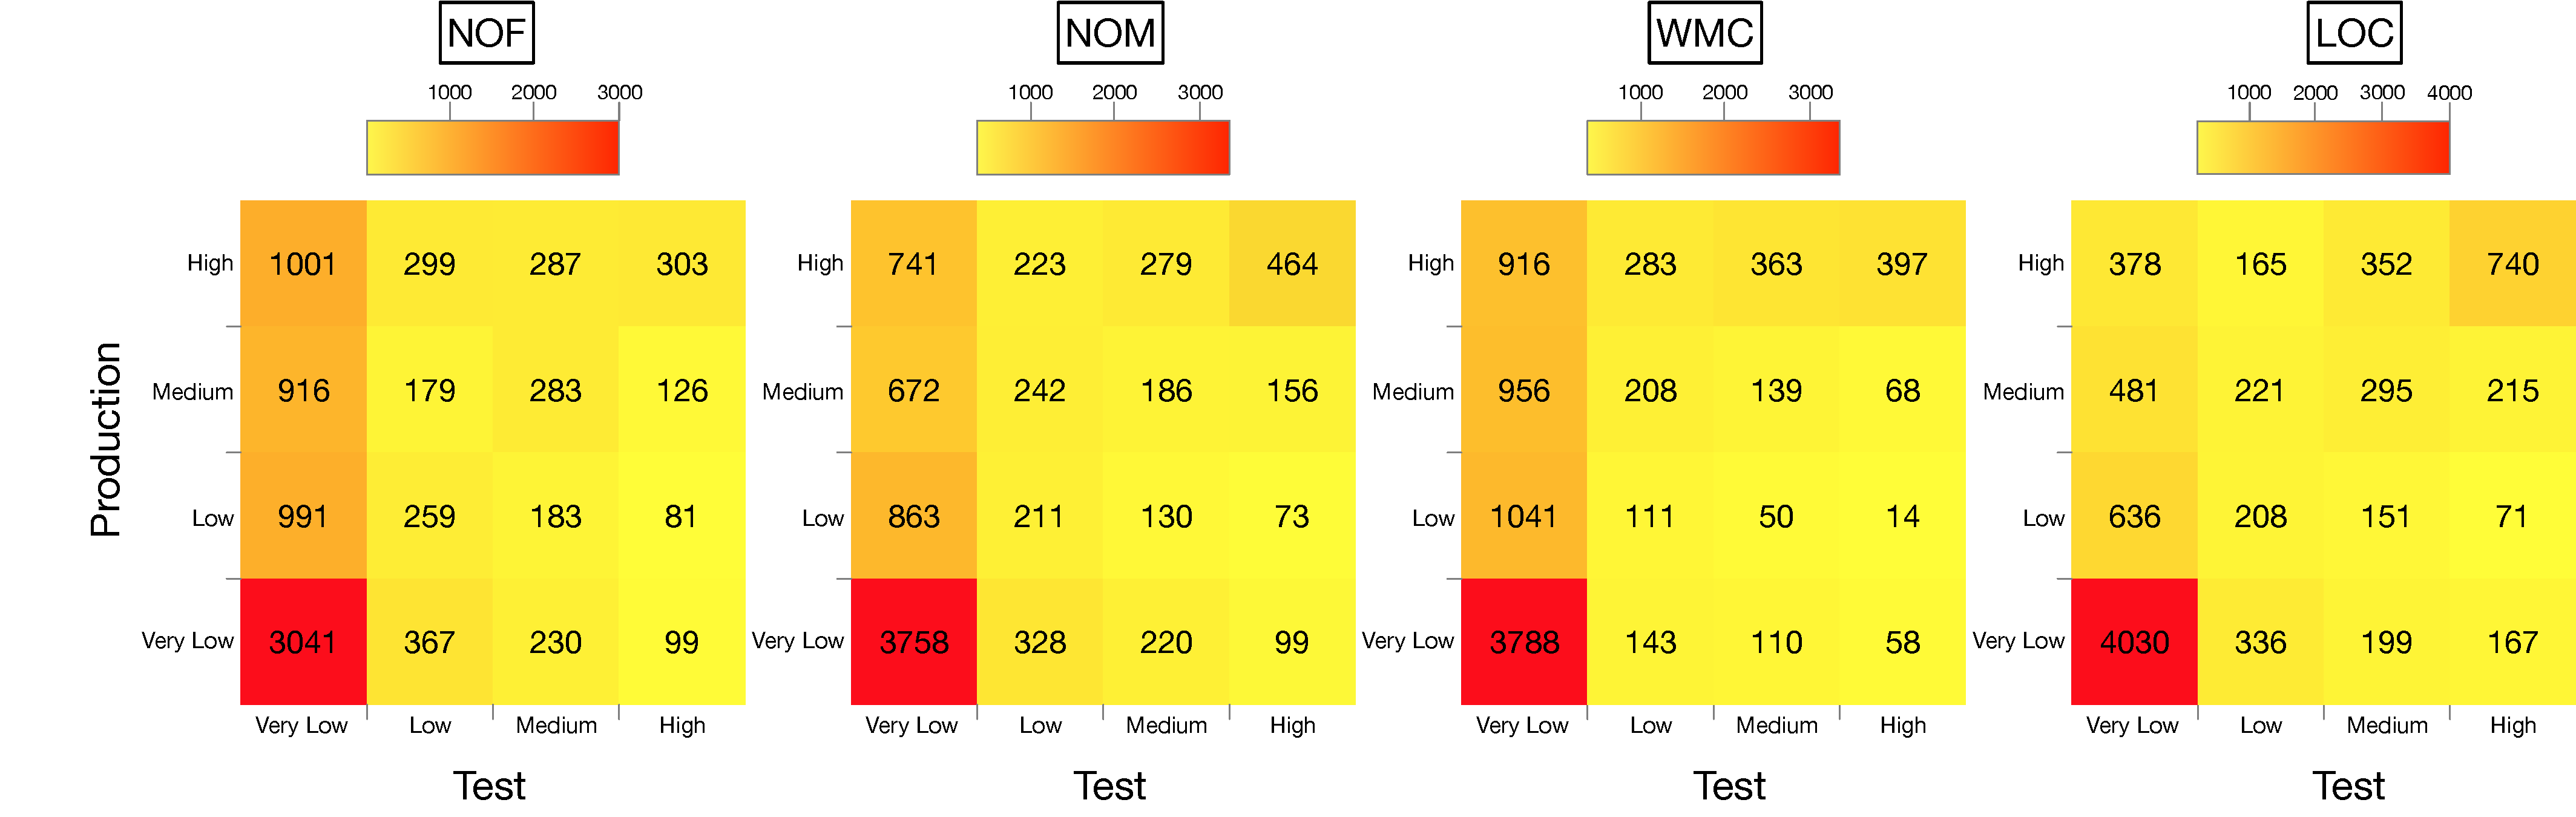
\includegraphics[width=\textwidth]{resources/heat_map.pdf}
    \caption{Categorization of test-production code class pairs for each metric. On the X-axis we find the test categories, while on Y-axis we find the categories of the corresponding production file.}
    \label{fig:heat_map}
\end{figure*}
